\documentclass[11pt,letterpaper]{article}

% Load some basic packages that are useful to have
% and that should be part of any LaTeX installation.
%
% be able to include figures
\usepackage{graphicx}
% get nice colors
\usepackage{xcolor}

% change default font to Palatino (looks nicer!)
\usepackage[latin1]{inputenc}
\usepackage{mathpazo}
\usepackage[T1]{fontenc}
% load some useful math symbols/fonts
\usepackage{latexsym,amsfonts,amsmath,amssymb}

% comfort package to easily set margins
\usepackage[top=1in, bottom=1in, left=1in, right=1in]{geometry}

% control some spacings
%
% spacing after a paragraph
\setlength{\parskip}{.15cm}
% indentation at the top of a new paragraph
\setlength{\parindent}{0.0cm}


\begin{document}

\begin{center}
\Large
Ay190 -- Worksheet 1\\
John Pharo\\
Date: \today \\
Agents of SHIELD: Anthony Alvarez, Cutter Coryell
\end{center}

\section*{Linear Regression}

\subsection*{(a)}

\begin{figure}[!htb]\centering
  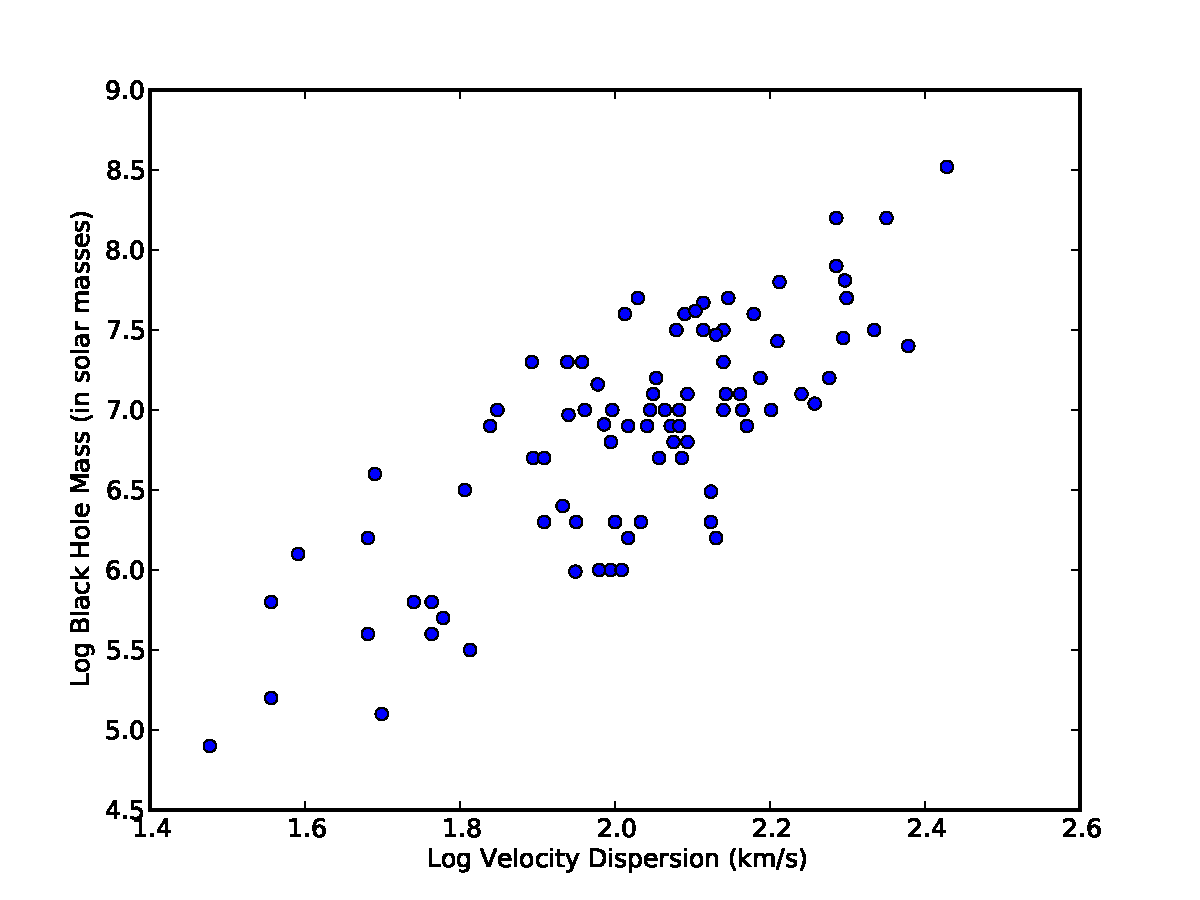
\includegraphics[width=1\textwidth]{PartA}
  \caption{Plot of black hole mass vs velocity dispersion, without error.}
  \end{figure}

\subsection*{(b)}

\[
\begin{array}{cccc}
a_1 & \sigma_{a_1} & a_2 & \sigma_{a_2} \\
0.93106967817676167 & 1.1158802783711324 & 2.925429008834183 & 0.54749789824558692
\end{array}
\]

\begin{figure}[!htb]\centering
  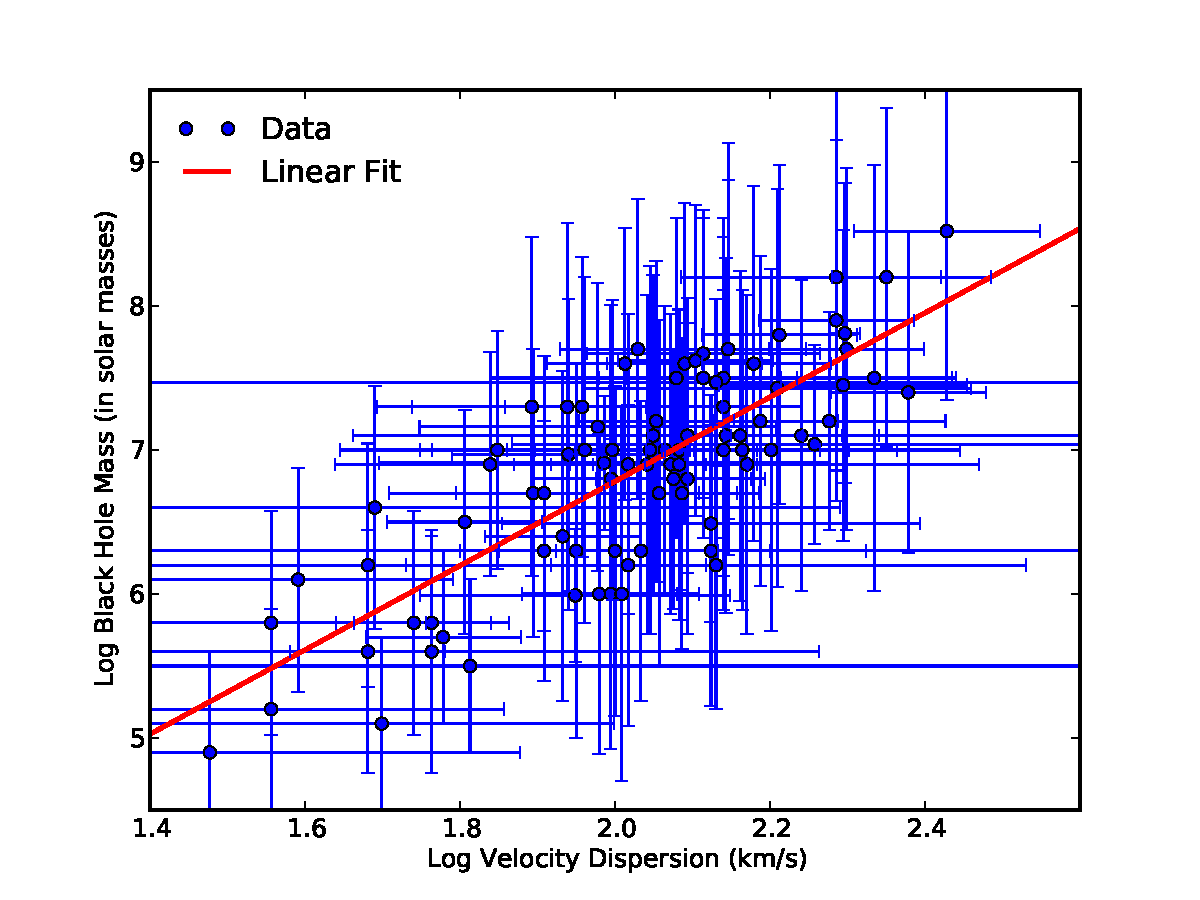
\includegraphics[width=1\textwidth]{PartB}
  \caption{Plot of black hole mass vs velocity dispersion, with error, and of a linear regression of the data, ignoring any error. The bounds are set to roughly match those of Figure 1 on the worksheet,, that we might compare to Greene and Ho. Thw two are fairly close, but my fit is shallower. However, the difference is likely within my errors for $a_1$ and $a_2$.}
  \end{figure}

\subsection*{(c)}

\[
\begin{array}{ccccc}
a_1 & \sigma_{a_1} & a_2 & \sigma_{a_2} & \chi^2 \\
0.45531570777031338 & 8.0153868647554827 & 3.0911839820456084 & 4.1349645712187764 & 0.30261736586887894
\end{array}
\]

Note that the errors in $a_1$ and $a_2$ are huge, larger than the values themselves, so the $\chi^2$ of the fit is less than one, meaning we haven't actually really fit the data. 

\begin{figure}[!htb]\centering
  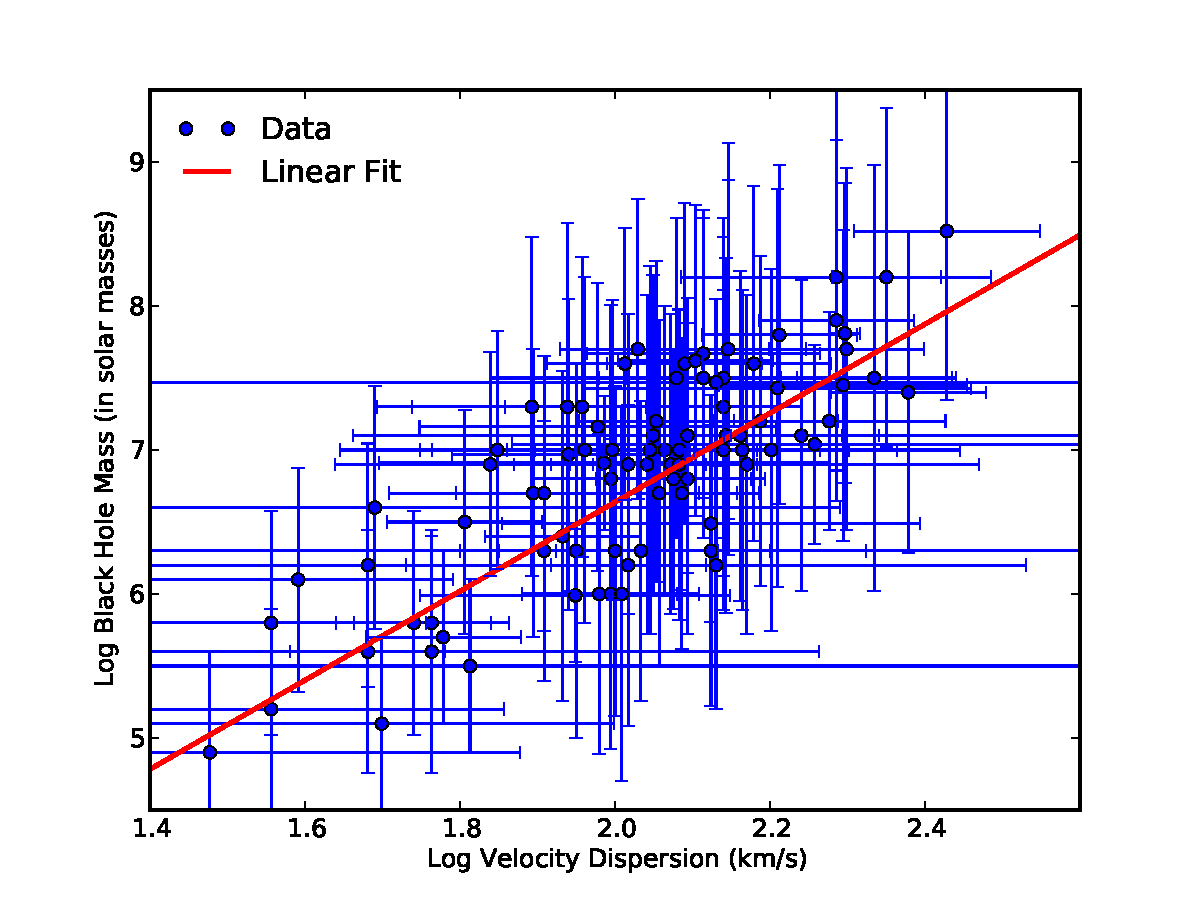
\includegraphics[width=1\textwidth]{PartC}
  \caption{Plot of black hole mass vs velocity dispersion, with error, and a linear regression of the data using both of those errors. This seems to have brought the fit down in the y-direction from part b.}
  \end{figure}

\end{document}
